% Taken from: https://mikedewar.wordpress.com/2009/02/25/latex-beamer-python-beauty/
\documentclass[12pt,english,pdf,xcolor=dvipsnames,aspectratio=169,handout]{beamer}\usepackage[]{graphicx}\usepackage[]{xcolor}
% maxwidth is the original width if it is less than linewidth
% otherwise use linewidth (to make sure the graphics do not exceed the margin)
\makeatletter
\def\maxwidth{ %
  \ifdim\Gin@nat@width>\linewidth
    \linewidth
  \else
    \Gin@nat@width
  \fi
}
\makeatother

\definecolor{fgcolor}{rgb}{0.345, 0.345, 0.345}
\newcommand{\hlnum}[1]{\textcolor[rgb]{0.686,0.059,0.569}{#1}}%
\newcommand{\hlstr}[1]{\textcolor[rgb]{0.192,0.494,0.8}{#1}}%
\newcommand{\hlcom}[1]{\textcolor[rgb]{0.678,0.584,0.686}{\textit{#1}}}%
\newcommand{\hlopt}[1]{\textcolor[rgb]{0,0,0}{#1}}%
\newcommand{\hlstd}[1]{\textcolor[rgb]{0.345,0.345,0.345}{#1}}%
\newcommand{\hlkwa}[1]{\textcolor[rgb]{0.161,0.373,0.58}{\textbf{#1}}}%
\newcommand{\hlkwb}[1]{\textcolor[rgb]{0.69,0.353,0.396}{#1}}%
\newcommand{\hlkwc}[1]{\textcolor[rgb]{0.333,0.667,0.333}{#1}}%
\newcommand{\hlkwd}[1]{\textcolor[rgb]{0.737,0.353,0.396}{\textbf{#1}}}%
\let\hlipl\hlkwb

\usepackage{framed}
\makeatletter
\newenvironment{kframe}{%
 \def\at@end@of@kframe{}%
 \ifinner\ifhmode%
  \def\at@end@of@kframe{\end{minipage}}%
  \begin{minipage}{\columnwidth}%
 \fi\fi%
 \def\FrameCommand##1{\hskip\@totalleftmargin \hskip-\fboxsep
 \colorbox{shadecolor}{##1}\hskip-\fboxsep
     % There is no \\@totalrightmargin, so:
     \hskip-\linewidth \hskip-\@totalleftmargin \hskip\columnwidth}%
 \MakeFramed {\advance\hsize-\width
   \@totalleftmargin\z@ \linewidth\hsize
   \@setminipage}}%
 {\par\unskip\endMakeFramed%
 \at@end@of@kframe}
\makeatother

\definecolor{shadecolor}{rgb}{.97, .97, .97}
\definecolor{messagecolor}{rgb}{0, 0, 0}
\definecolor{warningcolor}{rgb}{1, 0, 1}
\definecolor{errorcolor}{rgb}{1, 0, 0}
\newenvironment{knitrout}{}{} % an empty environment to be redefined in TeX

\usepackage{alltt}
\usepackage{etex}
\usetheme{default}
\beamertemplatenavigationsymbolsempty
\definecolor{fore}{RGB}{43,41,46}
\definecolor{back}{RGB}{255,255,255}
\definecolor{title}{RGB}{198,24,38}
\setbeamercolor{titlelike}{fg=title}
\setbeamercolor{normal text}{fg=fore,bg=back}
\usepackage{mathpazo}
\usepackage{amsmath}
\usepackage{multirow}
\renewcommand{\familydefault}{\rmdefault}
\usepackage[T1]{fontenc}
\usepackage{inputenc}
\usepackage{parskip}
\setcounter{secnumdepth}{3}
\setcounter{tocdepth}{3}
\usepackage{hyperref}
\hypersetup{pdfauthor={Constantin Manuel Bosancianu},
pdftitle={Advanced Topics in Applied Regression},
pdfsubject={Day 1: OLS basics & assumptions},
pdfkeywords={Budapest, ECPR, 2017, day 1, SSMT}}
\usepackage{babel}
\usepackage{graphicx}
\usepackage{subfigure}
\usepackage{palatino}
\usepackage{picture} % Put brace over items
% Defines a checkmark
\def\checkmark{\tikz\fill[scale=0.4,color=title](0,.35) -- (.25,0) -- (1,.7) -- (.25,.15) -- cycle;}
\setbeamertemplate{itemize items}{\checkmark}
% For table captions in Beamer
\usepackage[labelformat=empty]{caption}
\captionsetup[figure]{labelfont={color=fore}}
\captionsetup[table]{labelfont={color=fore}}
\usepackage{tikz, tikz-cd, animate}
\usetikzlibrary{shapes,backgrounds,trees}
\usetikzlibrary{decorations.pathreplacing}
\usepackage{pgfplots}
\pgfplotsset{compat=1.10}
\usepgfplotslibrary{fillbetween}
\usepackage{pgfplotstable}
\usepackage{wrapfig}
\usepackage{booktabs}
\usepackage{dcolumn}
\usepackage[sectionbib]{apacite}
\renewcommand{\bibliographytypesize}{\footnotesize}
% Set the design of the footer
\makeatletter
\setbeamercolor{author in head/foot}{fg=white, bg=title}
\setbeamercolor{date in head/foot}{fg=white, bg=title}
\setbeamercolor{institute in head/foot}{fg=white, bg=title}
\setbeamertemplate{footline}
{
  \leavevmode%
  \hbox{%
  \begin{beamercolorbox}[wd=.3333333\paperwidth,ht=2.25ex,dp=1ex,center]{author in head/foot}%
    \usebeamerfont{author in head/foot}\insertauthor
  \end{beamercolorbox}%
    \begin{beamercolorbox}[wd=.3333333\paperwidth,ht=2.25ex,dp=1ex,center]{institute in head/foot}%
    \usebeamerfont{institute in head/foot}Central European University, Budapest
  \end{beamercolorbox}%
  \begin{beamercolorbox}[wd=.3333333\paperwidth,ht=2.25ex,dp=1ex,right]{date in head/foot}%
    \usebeamerfont{date in head/foot}\insertshortdate{}\hspace*{2em}
    \insertframenumber{} / \inserttotalframenumber\hspace*{2ex}
  \end{beamercolorbox}}%
  \vskip0pt%
}
\makeatother
\title{Advanced Topics in Applied Regression}
\subtitle{Day 1: OLS basics \& assumptions}
\author{Constantin Manuel Bosancianu}
\institute{Doctoral School of Political Science \\ Central European University, Budapest\\\href{mailto:bosancianu@icloud.com}{bosancianu@icloud.com}}
\date{July 31, 2017}
\IfFileExists{upquote.sty}{\usepackage{upquote}}{}
\begin{document}
\maketitle
% PREAMBLE %
\section{Preamble}




\begin{frame}{Welcome!}

  Thanks for taking the class!\bigskip

  Reasoning:

  \begin{itemize}
  \item Some of these topics you have to have in your toolbox, e.g. interactions or fixed effects;
  \item Others you need so as to avoid more complex procedures, e.g. clustered SEs, which, \textit{in certain specific cases}, can obviate the need for MLM.
  \end{itemize}
  
\end{frame}




\begin{frame}{Setup}

  Lecture + lab, both of which will be highly interactive. Ask questions and bring examples from data sets or research projects that you are working on!\bigskip

  R syntax supplied by myself (usually the morning of the class).\bigskip

  We will make some \textit{moderate} use of statistical notation.
\end{frame}




\begin{frame}{Why notation?}

  You will encounter it in a lot of quantitative literature, so it's good to get familiar with it early.\bigskip

  Some statistical topics you will have to learn on your own, so it's best if you get used with the symbols which many books use.\bigskip

  It slows you down a bit in the short term, but makes things faster in the long term.

\end{frame}


\begin{frame}{Glossary (I)}

  \begin{itemize}
  \item $X$, $Y$: variables
  \item $\overline{X}$: mean of $X$
  \item $\sigma_X^2$: variance of $X$, computed as $\frac{\sum_{i=1}^n(x_i - \bar{x})^2}{n-1}$
  \item $n$: sample size
  \end{itemize}

\end{frame}



\begin{frame}{Glossary (II)}

  \begin{itemize}
  \item $cov(X,Y)$: covariance between $X$ and $Y$ 
  \begin{itemize}
    \item computed as $\frac{\sum\limits_{i=1}^n(x_i - \bar{x})(y_i - \bar{y})}{n-1}$
  \end{itemize}
  \item $r_{XY}$: correlation between $X$ and $Y$, if both are continuous variables\footnote{Other types of correlations have different symbols, such as $\rho$.}
  \begin{itemize}
    \item computed as $\frac{cov(X,Y)}{\sigma_x\sigma_y} = \frac{\frac{\sum\limits_{i=1}^n(x_i - \bar{x})(y_i - \bar{y})}{n-1}}{\sigma_x\sigma_y}$ 
  \end{itemize}
  \end{itemize}

\end{frame}



\begin{frame}
\begin{center}
    \Huge Regression recap
\end{center}
\end{frame}


\begin{frame}{Standard multiple regression}

\begin{equation}
Y = a + b_1X_1 + b_2X_2 + \dots + b_kX_k + e
\end{equation}

Each individual in the sample has a different value on $Y$ and $X_1$, $X_2$, \dots, $X_k$.\bigskip

This means that the $e$s (errors, residuals) will also be different for each individual.

\end{frame}


\begin{frame}{Visualizing simple regression}

\begin{figure}
\centering
\begin{tikzpicture}[scale=0.9]
\begin{axis}[
xlabel=X, % label x axis
ylabel=Y, % label y axis
axis lines=left, %set the position of the axes
xmin=0, xmax=5, % set the min and max values of the x-axis
ymin=0, ymax=10, % set the min and max values of the y-axis
clip=false
]

\draw [very thick] (50,20) -- (400,80);
\draw [dotted, ->, >=stealth] (200,0)--(200,44.5);
\draw [dotted, ->, >=stealth] (300,0)--(300,61.5);
\node [circle, fill, inner sep=-2pt] (A) at (200,45.7) [label=\scriptsize{$\hat{y_1}$}] {};
\node [circle, fill, inner sep=-2pt] (B) at (300,62.7) [label=\scriptsize{$\hat{y_2}$}] {};
\draw [thick,->,>=stealth] (200,10)--(300,10) node [midway,above] {\tiny{1-unit}};
\draw [thick,->,>=stealth] (200,10)--(300,10) node [midway,below] {\tiny{difference}};
\draw [dotted, ->, >=stealth] (200,45.5)--(0,45.5);
\draw [dotted, ->, >=stealth] (300,62.5)--(0,62.5);
\draw[decorate,decoration={brace, mirror}] (10,45.5) -- node[right] {\tiny{$b$ change}} (10,62.5);
% Draw the intercept line
\draw [very thick, dotted] (0,11.42857) -- (50,20);
\draw[decorate,decoration={brace}] (-5,0) -- node[left] {\tiny{$a$}} (-5,11.42857);
\end{axis}
\end{tikzpicture}
\caption{Slope interpretation (I call the predicted value of Y for $x_i$ as $\hat{y}_i$)}
\label{fig:fig-01}
\end{figure}

\end{frame}


\begin{frame}{Visualizing multiple regression}

\begin{figure}
\centering
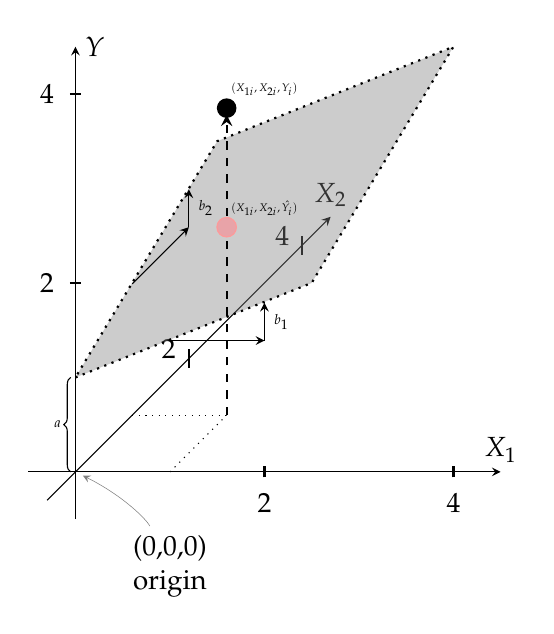
\begin{tikzpicture}[x=1.2cm,y=1.2cm,z=0.72cm,>=stealth]
% The axes
\draw[->] (xyz cs:x=-0.5) -- (xyz cs:x=4.5) node[above] {$X_1$};
\draw[->] (xyz cs:y=-0.5) -- (xyz cs:y=4.5) node[right] {$Y$};
\draw[->] (xyz cs:z=-0.5) -- (xyz cs:z=4.5) node[above] {$X_2$};
% The thick ticks
\foreach \coo in {2,4}
{
  \draw[thick] (\coo,-2pt) -- (\coo,2pt) node[below=6pt] {\coo};
  \draw[thick] (-2pt,\coo) -- (2pt,\coo) node[left=6pt] {\coo};
  \draw[thick] (xyz cs:y=-0.1pt,z=\coo) -- (xyz cs:y=0.1pt,z=\coo) node[left=1pt] {\coo};
}

% The origin
\node[align=center] at (1,-1) (ori) {(0,0,0)\\\text{origin}};
\draw[->,help lines,shorten >=3pt] (ori) .. controls (0.75,-0.5) and (0.5,-0.25) .. (0,0,0);

% Draw the plane
\path[fill=gray, dotted, thick, draw=black, fill opacity=0.4] (0,1,0)--(2.5,2,0)--(2.5,3,2.5)--(0,2,2.5)--(0,1,0);
\draw[->, >=stealth] (1,1.39,0) -- (2,1.39,0);
\draw[->, >=stealth] (2,1.39,0) -- (2,1.79,0) node [midway, right] {\tiny{$b_1$}};
\draw[->, >=stealth] (0,1.39,1) -- (0,1.39,2);
\draw[->, >=stealth] (0,1.39,2) -- (0,1.79,2) node [midway, right] {\tiny{$b_2$}};
\draw[decorate,decoration={brace}] (-0.05,0,0) -- node[left] {\tiny{$a$}} (-0.05,1,0);

% Draw one point as an example
\node[circle, fill=black, scale=0.75] at (1,3.25,1) {};
\node[fill=none, scale=0.8] at (1.4,3.45,1) {\tiny{$(X_{1i},X_{2i},Y_i)$}};
\draw[->, dashed, thick, >=stealth] (1,0,1) -- (1,3.18,1);
\draw[dotted] (0,0,1) -- (1,0,1);
\draw[dotted] (1,0,0) -- (1,0,1);
\node[circle, fill=title!40, draw=red!40, scale=0.75] at (1,1.99,1) {};
\node[fill=none, scale=0.8] at (1.4,2.19,1) {\tiny{$(X_{1i},X_{2i},\hat{Y_i})$}};
\end{tikzpicture}
\caption{Two predictors (adapted from \citeNP{fox2008})}
\end{figure}

\end{frame}



\begin{frame}{Model fit}

Most common is $R^2$, interpreted as the share of the variance in $Y$ explained by the influence of $X_1$, $X_2$, \dots $X_k$.\bigskip

\begin{equation}
Adjusted\; R^2:\tilde{R}^2 = 1 - \frac{(1-R^2)(n-1)}{n-k-1}
\end{equation}

For the adjusted $R^2$ \textsf{R} uses the ``Wherry Formula $-1$''.\bigskip

\begin{equation}
Residual\; SE: \sigma_e = \sqrt{\frac{\sum_{i=1}^ne_i^2}{n-k-1}}
\end{equation}

$\sigma_e$ is an alternative measure of fit, interpreted as a sort of ``average residual'' (sadly, it's often not reported).

\end{frame}



\begin{frame}{Inference with regression}

For simple regression:

\begin{equation}
V(b) = \frac{\sigma_e^2}{\sum_{i=1}^n(x_i - \bar{x})^2} = \frac{\sigma_e^2}{(n-1)\sigma_x^2}
\end{equation}

\begin{itemize}
\item larger $n$ means smaller $V(b)$;
\item as $\sigma_e^2$ increases, so does $V(b)$;
\item as $\sum_{i=1}^{n}(x_i - \bar{x})^2$ increases, $V(b)$ gets smaller.
\end{itemize}

\end{frame}


\begin{frame}{Inference for multiple regression}

\begin{equation}
V(b_j) = \underbrace{\frac{1}{1 - R_j^2}}_\text{VIF} \times \frac{\sigma_e^2}{\sum_{i=1}^n(x_{j} - \bar{x_j})^2}
\end{equation}

The second part is the same as for simple regression. The first part is called the \textit{variance inflation factor} (VIF).\bigskip

$R_j^2$ is the model fit from a regression of $X_j$ on all the other $X$s (predictors) in the model.

\end{frame}




\section{Introduction}

\begin{frame}
\begin{center}
    \Huge Introduction
\end{center}
\end{frame}


\begin{frame}{Why assumptions}
  We can only ``trust'' the estimated $a$, $b$s and SEs if the data follows certain specifications.\bigskip

  Without these, we can't be sure that the population effects are the same as the estimated sample effects.
  
\end{frame}



\begin{frame}{MIA (most important assumptions)}
  The residuals:

  \begin{enumerate}
  \item Average of the $e$s is 0 along the length of $X$s: $E(e | x_i)=0$;
  \item Variance is constant along the length of $X$s: $V(e | x_i) = \sigma_e^2$. This is also called the assumption of ``homoskedasticity'';\footnote{The violation of this assumption if called ``heteroskedasticity''. Sometimes you encounter this term with a ``c'' instead of a ``k''.}
  \item Errors are normally distributed: $e_i \sim \mathcal{N}(0, \sigma_e^2)$;
  \item Errors are independent from each other: $cov(e_i,e_j)=0$, for any $i \neq j$;
  \item Predictors are measured without error, and are independent of the errors: $cov(X,e)=0$.
  \end{enumerate}
  
\end{frame}


\section{Linearity}


\begin{frame}
\begin{center}
    \Huge Linearity
\end{center}
\end{frame}


\begin{frame}[fragile]{Linearity assumption}

\begin{columns}[T]
    \begin{column}{.4\textwidth}
     \begin{block}{}
\footnotesize{
Two understandings:

\begin{itemize}
\item The bivariate relationship between $X$ and $Y$ is linear;
\item The mean of $e_i$ is 0 along the length of $X$.
\end{itemize}
}
    \end{block}
    \end{column}
    \begin{column}{.6\textwidth}
    \begin{block}{}
\begin{figure}
\centering
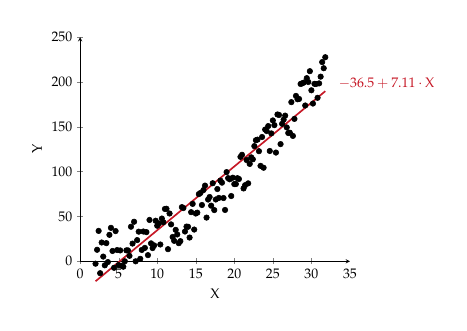
\begin{tikzpicture}[scale=0.5]
% For the regression graph below
\pgfmathsetseed{1144} % set the random seed
\pgfplotstableset{ % Define the equations for x and y
	create on use/x/.style={create col/expr={2+0.2*\pgfplotstablerow}},
	create on use/y/.style={create col/expr={(0.2*\thisrow{x}*\thisrow{x})+10)+25*rand}}
}
% create a new table with 150 rows and columns x and y:
\pgfplotstablenew[columns={x,y}]{150}\loadedtable
\begin{axis}[
xlabel=X, % label x axis
ylabel=Y, % label y axis
axis lines=left, %set the position of the axes
xmin=0, xmax=35, % set the min and max values of the x-axis
ymin=0, ymax=250, % set the min and max values of the y-axis
clip=false
]

\addplot [only marks] table {\loadedtable};
\addplot [no markers, very thick, color=title] table [y={create col/linear regression={y=y}}] {\loadedtable} node [anchor=west, xshift=0.2cm, yshift=0.2cm] {$\pgfmathprintnumber[precision=2]{\pgfplotstableregressionb} + \pgfmathprintnumber[precision=2, fixed zerofill]{\pgfplotstableregressiona} \cdot \mathrm{X}$};
\end{axis}
\end{tikzpicture}
\caption{Nonlinear relationship}
\label{fig:fig-01}
\end{figure}
    \end{block}
    \end{column}
  \end{columns}

The two are equivalent.

\end{frame}



\subsection{Diagnosis}


\begin{frame}{Diagnosing linearity}
Plotting $X$s against $Y$ can detect some cases, but can miss some others for multiple regression.\bigskip

The standard way is the \textit{component-plus-residual plot}.\footnote{In other texts you will encounter it as the \textit{partial-residual} plot.}\bigskip

For each observation for a specific predictor, compute

\begin{equation}
e_i^{(k)} = e_i + b_kX_k
\end{equation}

This is called the \textit{partial residual}. Plotting $e_i^{(k)}$ against $X_k$ should reveal any nonlinearity.

\end{frame}


\begin{frame}{Example: infant mortality}




\begin{table}
\caption{Model for infant mortality}
\begin{center}
\begin{footnotesize}
\begin{tabular}{l D{.}{.}{3.5}}
\toprule
 & \multicolumn{1}{c}{DV: Infant mortality} \\
\midrule
(Intercept)              & 19.55^{***} \\
                         & (1.40)      \\
GDP/capita (1,000s)      & -0.49^{***} \\
                         & (0.08)      \\
Sub-Saharan Africa (yes) & 35.39^{***} \\
                         & (2.65)      \\
\midrule
R$^2$                    & 0.63        \\
Adj. R$^2$               & 0.63        \\
Num. obs.                & 183         \\
\bottomrule
\multicolumn{2}{l}{\tiny{$^{***}p<0.001$; $^{**}p<0.01$; $^{*}p<0.05$. GDP/capita rescaled by subtracting 5,000 USD.}}
\end{tabular}
\end{footnotesize}
\label{tab:tab-02}
\end{center}
\end{table}


\end{frame}


\begin{frame}{Example: infant mortality}



\begin{figure}
  \centering
  \includegraphics[scale=0.375]{../04-graphs/01-01.pdf}
  \caption{\label{fig:fig-02} Component-plus-residual plot for infant mortality regression (solid line is a \textit{lowess} fit).}
\end{figure}

\end{frame}



\subsection{Solution}

\begin{frame}{Addressing linearity}
A standard solution is to transform one of the predictors; in our case, this is GDP/capita.\bigskip


\begin{table}
\begin{center}
\begin{scriptsize}
\begin{tabular}{l D{.}{.}{3.5} D{.}{.}{3.5}}
\toprule
 & \multicolumn{1}{c}{Model 1} & \multicolumn{1}{c}{Model 2} \\
\midrule
(Intercept)         & 19.55^{***} & 87.86^{***} \\
                    & (1.40)      & (6.29)      \\
GDP/capita (1,000s) & -0.49^{***} &             \\
                    & (0.08)      &             \\
Sub-Saharan Africa  & 35.39^{***} & 24.53^{***} \\
                    & (2.65)      & (2.52)      \\
log(GDP/capita)     &             & -8.31^{***} \\
                    &             & (0.71)      \\
\midrule
R$^2$               & 0.63        & 0.74        \\
Adj. R$^2$          & 0.63        & 0.74        \\
Num. obs.           & 183         & 183         \\
\bottomrule
\multicolumn{3}{l}{\tiny{$^{***}p<0.001$; $^{**}p<0.01$; $^{*}p<0.05$. GDP/capita used in its original form.}}
\end{tabular}
\end{scriptsize}
\caption{Comparison of models---problematic nonlinearity for infant mortality regression}
\label{tab:tab-03}
\end{center}
\end{table}


\end{frame}


\begin{frame}{Addressing linearity}



\begin{figure}
  \centering
  \includegraphics[scale=0.375]{../04-graphs/01-02.pdf}
  \caption{\label{fig:fig-03} Component-plus-residual plot for infant mortality regression, with changed specification.}
\end{figure}

\end{frame}



\begin{frame}{Addressing linearity (cont.)}

  Another strategy would be to change the functional form of the model.\bigskip

  In our case, this would mean adding both GDP/capita and a squared GDP/capita (the latter is called a \textit{quadratic term}).\bigskip

  The squared version can be considered a multiplicative interaction\footnote{More on this Wednesday.}, which would show how the slope of GDP/capita changes depending on \dots GDP/capita.

\end{frame}



\subsection{Transformations}

\begin{frame}{Mosteller and Tukey's rules}

\begin{figure}[!ht]
\centering
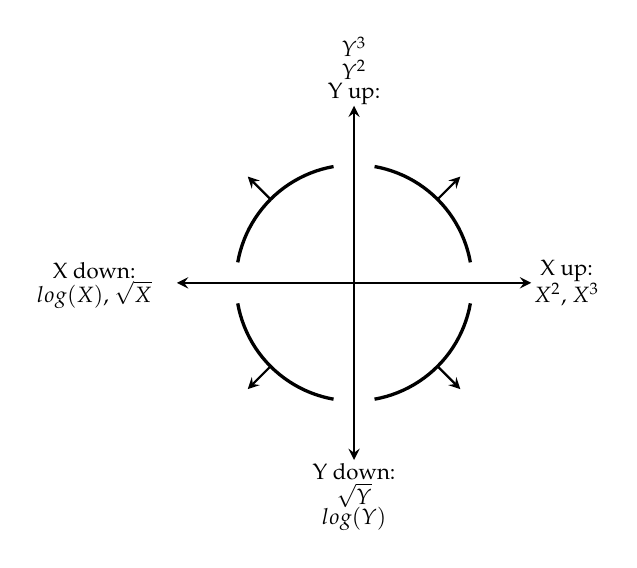
\begin{tikzpicture}[scale=1.5]
% Axes
\draw[thick, black, <->, >=stealth] (0,-1.5)--(0,1.5);
\draw[thick, black, <->, >=stealth] (-1.5,0)--(1.5,0);
% Arcs
\draw [black, very thick, domain=10:80] plot ({cos(\x)}, {sin(\x)});
\draw [black, very thick, domain=100:170] plot ({cos(\x)}, {sin(\x)});
\draw [black, very thick, domain=190:260] plot ({cos(\x)}, {sin(\x)});
\draw [black, very thick, domain=280:350] plot ({cos(\x)}, {sin(\x)});
% Arrows
\draw[thick, black, ->, >=stealth] (0.7071068,0.7071068)--(0.9,0.9);
\draw[thick, black, ->, >=stealth] (0.7071068,-0.7071068)--(0.9,-0.9);
\draw[thick, black, ->, >=stealth] (-0.7071068,-0.7071068)--(-0.9,-0.9);
\draw[thick, black, ->, >=stealth] (-0.7071068,0.7071068)--(-0.9,0.9);
% Markings
\node[draw=none] at (0,1.6) {\footnotesize{Y up:}};
\node[draw=none] at (0,1.8) {\footnotesize{$Y^2$}};
\node[draw=none] at (0,2.0) {\footnotesize{$Y^3$}};
\node[draw=none] at (0,-1.6) {\footnotesize{Y down:}};
\node[draw=none] at (0,-1.8) {\footnotesize{$\sqrt{Y}$}};
\node[draw=none] at (0,-2.0) {\footnotesize{$log(Y)$}};
\node[draw=none] at (1.8,0.1) {\footnotesize{X up:}};
\node[draw=none] at (1.8,-0.1) {\footnotesize{$X^2$, $X^3$}};
\node[draw=none] at (-2.2,0.1) {\footnotesize{X down:}};
\node[draw=none] at (-2.2,-0.1) {\footnotesize{$log(X)$, $\sqrt{X}$}};
\end{tikzpicture}
\caption{Mosteller and Tukey's \citeyear[p.~84]{mosteller1977} set of rules for transformations.}
\label{fig:fig-04}
\end{figure}

\end{frame}



\begin{frame}{Transformations for univariate distributions}

\begin{columns}[T]
    \begin{column}{.5\textwidth}
     \begin{block}{Positive skew}
       \footnotesize
       Moderate: $NEW=\sqrt{OLD}$

       Substantive: $NEW=\log_{10}OLD$

       Substantive (with 0s): $NEW=\log_{10}(OLD + c_1)$
     \end{block}
    \end{column}
    \begin{column}{.5\textwidth}
    \begin{block}{Negative skew}
      \footnotesize
      Moderate: $NEW = \sqrt{c_2 - OLD}$

      Substantive: $NEW = \log_{10}(c_2 - OLD)$
    \end{block}
    \end{column}
  \end{columns}

  $c_1$: constant added so that smallest value is 1.\bigskip

  $c_2$: constant from which old values are subtracted so that smallest new value is 1.\bigskip

  Naturally, transformations also imply a change in interpretation of the transformed variable.

\end{frame}




\section{Homoskedasticity}

\begin{frame}
\begin{center}
    \Huge Homoskedasticity
\end{center}
\end{frame}


\begin{frame}{Homoskedasticity}
The spread of $e_i$ should be constant along the length of $\hat{Y}$.\bigskip

\begin{figure}
\includegraphics{../04-graphs/01-03.pdf}
\end{figure}

\end{frame}



\begin{frame}[fragile]{Heteroskedasticity}

\begin{figure}
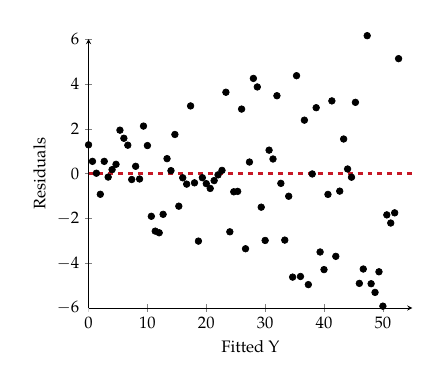
\begin{tikzpicture}[scale=0.6]
% For the regression graph below
\pgfmathsetseed{1146} % set the random seed
\pgfplotstableset{ % Define the equations for x and y
	create on use/x/.style={create col/expr={\pgfplotstablerow/1.5}},
	create on use/y/.style={create col/expr={(1.5 + \pgfplotstablerow/15)*rand}}
}
% create a new table with 80 rows and columns x and y:
\pgfplotstablenew[columns={x,y}]{80}\loadedtable
\begin{axis}[
xlabel=Fitted Y, % label x axis
ylabel=Residuals, % label y axis
axis lines=left, %set the position of the axes
xmin=0, xmax=55, % set the min and max values of the x-axis
ymin=-6, ymax=6, % set the min and max values of the y-axis
clip=false
]

\addplot [only marks] table {\loadedtable};
\draw[ultra thick, dashed, color=title] (axis cs:\pgfkeysvalueof{/pgfplots/xmin},0) -- (axis cs:\pgfkeysvalueof{/pgfplots/xmax},0);
\end{axis}
\end{tikzpicture}
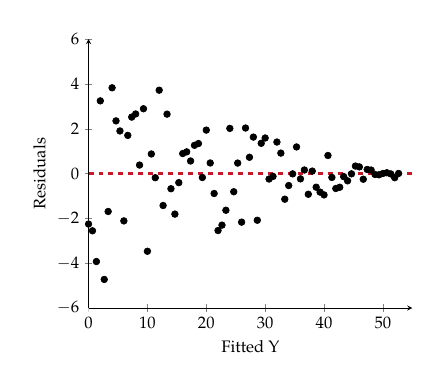
\begin{tikzpicture}[scale=0.6]
% For the regression graph below
\pgfmathsetseed{1147} % set the random seed
\pgfplotstableset{ % Define the equations for x and y
	create on use/x/.style={create col/expr={\pgfplotstablerow/1.5}},
	create on use/y/.style={create col/expr={(5 - \pgfplotstablerow/15)*rand}}
}
% create a new table with 80 rows and columns x and y:
\pgfplotstablenew[columns={x,y}]{80}\loadedtable
\begin{axis}[
xlabel=Fitted Y, % label x axis
ylabel=Residuals, % label y axis
axis lines=left, %set the position of the axes
xmin=0, xmax=55, % set the min and max values of the x-axis
ymin=-6, ymax=6, % set the min and max values of the y-axis
clip=false
]

\addplot [only marks] table {\loadedtable};
\draw[ultra thick, dashed, color=title] (axis cs:\pgfkeysvalueof{/pgfplots/xmin},0) -- (axis cs:\pgfkeysvalueof{/pgfplots/xmax},0);
\end{axis}
\end{tikzpicture}
\end{figure}

$a$ and $b$s are unbiased, but their SEs are imprecise, which means significance tests are affected.

\end{frame}



\subsection{Diagnosis}

\begin{frame}{Diagnosing heteroskedasticity}

\begin{figure}
\centering
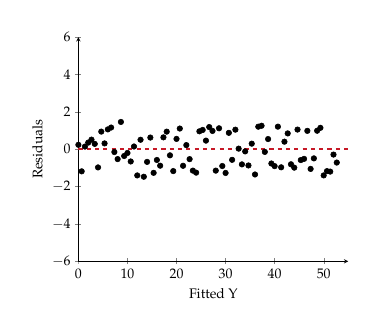
\begin{tikzpicture}[scale=0.5]
% For the regression graph below
\pgfmathsetseed{1145} % set the random seed
\pgfplotstableset{ % Define the equations for x and y
	create on use/x/.style={create col/expr={\pgfplotstablerow/1.5}},
	create on use/y/.style={create col/expr={1.5*rand}}
}
% create a new table with 80 rows and columns x and y:
\pgfplotstablenew[columns={x,y}]{80}\loadedtable
\begin{axis}[
xlabel=Fitted Y, % label x axis
ylabel=Residuals, % label y axis
axis lines=left, %set the position of the axes
xmin=0, xmax=55, % set the min and max values of the x-axis
ymin=-6, ymax=6, % set the min and max values of the y-axis
clip=false
]

\addplot [only marks] table {\loadedtable};
\draw[ultra thick, dashed, color=title] (axis cs:\pgfkeysvalueof{/pgfplots/xmin},0) -- (axis cs:\pgfkeysvalueof{/pgfplots/xmax},0);
\end{axis}
\end{tikzpicture}
\end{figure}

Is $\sigma_e^2$ constant?

\begin{itemize}
\item a plot of studentized residuals versus fitted values ($\hat{Y}$);\footnote{Using Y would result in a tilted plot, which is a bit harder to interpret; $\hat{Y}$ and the studentized residuals are uncorrelated, though, so the plot will be ``flat''.}
\item a plot of studentized residuals versus predictors ($X_k$).
\end{itemize}

\end{frame}


\begin{frame}[fragile]{Example: California counties in 1992}

\begin{figure}
	\centering
	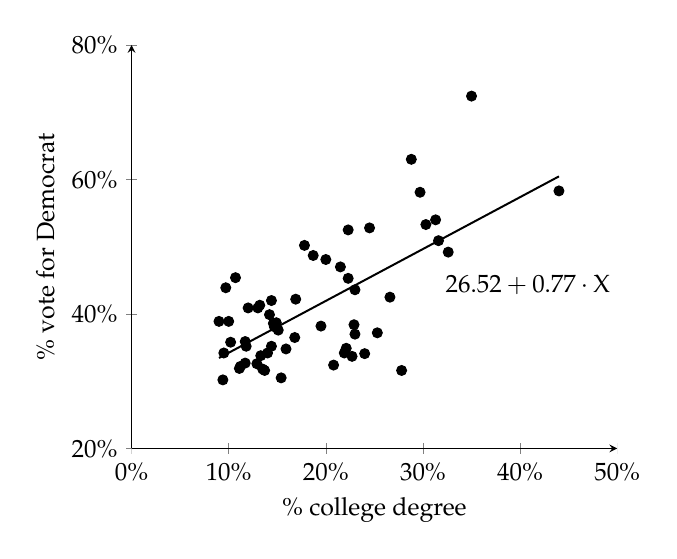
\begin{tikzpicture}[scale=0.9]
	\pgfplotstableread{
x y
28.7999992370605	63
24	34.0999984741211
14	34.2000007629395
19.5	38.2000007629395
14.3999996185303	35.2000007629395
11.1000003814697	31.8999996185303
31.6000003814697	50.9000015258789
10	38.9000015258789
20.7999992370605	32.4000015258789
16.8999996185303	42.2000007629395
9.39999961853027	30.2000007629395
20	48.0999984741211
9.69999980926514	43.9000015258789
13.5	31.7999992370605
13.3000001907349	33.7999992370605
9	38.9000015258789
10.6999998092651	45.4000015258789
11.6999998092651	32.7000007629395
22.2999992370605	52.5
11.6999998092651	35.9000015258789
44	58.2999992370605
16.7999992370605	36.5
17.7999992370605	50.2000007629395
12	40.9000015258789
11.1999998092651	32.2000007629395
21.8999996185303	34.2000007629395
21.5	47
22.2999992370605	45.2999992370605
22.1000003814697	34.9000015258789
27.7999992370605	31.6000003814697
22.7000007629395	33.7000007629395
15.1000003814697	37.5999984741211
14.6000003814697	38.5999984741211
23	43.5999984741211
14.3999996185303	42
14.8999996185303	38.7000007629395
25.2999992370605	37.2000007629395
35	72.4000015258789
13.1999998092651	41.2999992370605
22.8999996185303	38.4000015258789
31.2999992370605	54
26.6000003814697	42.5
32.5999984741211	49.2000007629395
29.7000007629395	58.0999984741211
13.6999998092651	31.6000003814697
15.8999996185303	34.7999992370605
14.1999998092651	39.9000015258789
18.7000007629395	48.7000007629395
24.5	52.7999992370605
13	40.9000015258789
15.3999996185303	30.5
10.1999998092651	35.7999992370605
12.8999996185303	32.5999984741211
11.8000001907349	35.2000007629395
14.6999998092651	38.0999984741211
23	37
30.2999992370605	53.2999992370605
9.5	34.2000007629395
}\loadedtable

	\begin{axis}[
	xlabel=\% college degree, % label x axis
	ylabel=\% vote for Democrat, % label y axis
	axis lines=left, %set the position of the axes
	xmin=0, xmax=50, % set the min and max values of the x-axis
	ymin=20, ymax=80, % set the min and max values of the y-axis
  xticklabel={\pgfmathparse{\tick}\pgfmathprintnumber{\pgfmathresult}\%},
  yticklabel={\pgfmathparse{\tick}\pgfmathprintnumber{\pgfmathresult}\%},
	clip=false
	]
	
 \addplot [only marks] table {\loadedtable};
 \addplot [no markers, thick, title] table [y={create col/linear regression={y=y}}] {\loadedtable} node [anchor=west, xshift=3cm, yshift=1cm] {$\pgfmathprintnumber[precision=2]{\pgfplotstableregressionb} + \pgfmathprintnumber[precision=2, fixed zerofill]{\pgfplotstableregressiona} \cdot \mathrm{X}$};
	\end{axis}
	\end{tikzpicture}
	\caption{OLS estimates: education and vote choice (CA 1992)}
\end{figure}

\end{frame}



\begin{frame}{Example: California counties in 1992}





\begin{figure}
\includegraphics[width=0.48\textwidth]{../04-graphs/01-04.pdf}
\includegraphics[width=0.48\textwidth]{../04-graphs/01-05.pdf}
\end{figure}

No clear evidence of heteroskedasticity.\bigskip

Take another case: average Boston house prices, at the neighborhood level. The goal is to understand what influences the price.

\end{frame}


\begin{frame}{Example: Boston house prices}


\begin{table}
\begin{center}
\begin{footnotesize}
\begin{tabular}{l D{.}{.}{3.6}}
\toprule
 & \multicolumn{1}{c}{DV: House price (ave.)} \\
\midrule
(Intercept)        & -42.757^{***} \\
                   & (9.620)       \\
Average num. rooms & 10.139^{***}  \\
                   & (1.568)       \\
\midrule
R$^2$              & 0.471         \\
Adj. R$^2$         & 0.460         \\
Num. obs.          & 49            \\
\bottomrule
\multicolumn{2}{l}{\tiny{$^{***}p<0.001$; $^{**}p<0.01$; $^{*}p<0.05$}}
\end{tabular}
\end{footnotesize}
\caption{Predicting house price using number of rooms}
\label{table:coefficients}
\end{center}
\end{table}


\end{frame}


\begin{frame}{Example: Boston house prices}



\begin{figure}
\includegraphics[width=0.48\textwidth]{../04-graphs/01-06.pdf}
\includegraphics[width=0.48\textwidth]{../04-graphs/01-07.pdf}
\end{figure}

Clear heteroskedasticity: the variance in the middle of the plot is considerably larger than at the left edge.

\end{frame}



\subsection{Solutions}

\begin{frame}{Addressing heteroskedasticity}

None of the solutions are particularly simple.\bigskip

The first is \textit{Weighted Least Squares}---the quantities $\frac{1}{e_i}$ are used as weights to re-estimate the model.\bigskip

Observations with large $e_i$ are down-weighted in this setup.

\end{frame}



\begin{frame}{Addressing heteroskedasticity (cont.)}

Since the SEs are the problem, we can do a correction on the SEs.\bigskip

``Huber--White standard errors'', ``robust standard errors'', ``sandwich estimator'' \cite{huber1967,white1980}.\bigskip

If the heteroskedasticity is caused by omitted variables in the model specification, though, then the Huber--White correction doesn't give us much.\bigskip

In this case, Huber-White SEs provide accurate estimates of uncertainty for wrong estimates of effect \cite{freedman2006}.

\end{frame}



\begin{frame}[fragile]{Addressing heteroskedasticity (cont.)}

Use background knowledge about the topic to find whether heteroskedasticity is due to an omitted variable.\bigskip

In our case, I omitted a dummy variable and an interaction, since the data was collected from 2 different towns.\footnote{And the slope is different in the two towns.}\bigskip

Including these two predictors in the model results in a better distribution of the errors.

\end{frame}



\begin{frame}[fragile]{Addressing heteroskedasticity (cont.)}

You ought not be deterred by small differences in residual variances.\bigskip

Results are problematic only when $\sigma_e$ at its highest level is about 2 or 3 times as large as $\sigma_e$ at its lowest level \cite{fox2008}.

\end{frame}






\section{Normality of errors}

\begin{frame}
\begin{center}
    \Huge Normality of errors
\end{center}
\end{frame}


\begin{frame}[fragile]{Normality}

\begin{figure}[ht]
  \centering
  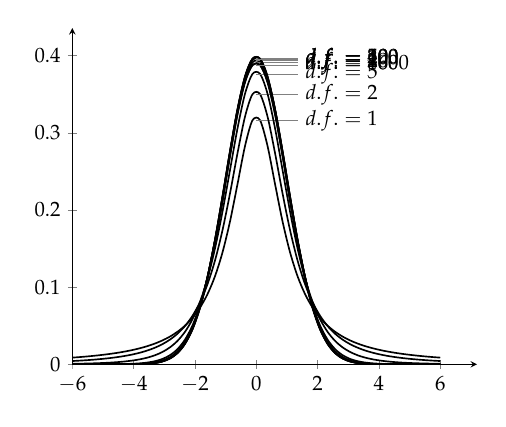
\begin{tikzpicture}[
    declare function={gamma(\z)=
    2.506628274631*sqrt(1/\z)+ 0.20888568*(1/\z)^(1.5)+ 0.00870357*(1/\z)^(2.5)- (174.2106599*(1/\z)^(3.5))/25920- (715.6423511*(1/\z)^(4.5))/1244160)*exp((-ln(1/\z)-1)*\z;},
    declare function={student(\x,\n)= gamma((\n+1)/2.)/(sqrt(\n*pi) *gamma(\n/2.)) *((1+(\x*\x)/\n)^(-(\n+1)/2.));},
    scale=0.75
]

\begin{axis}[
    axis lines=left,
    enlargelimits=upper,
    samples=50
]
\pgfplotsinvokeforeach{1,2,5,20,50,100,200,400,800,1600}{
    \addplot [thick, smooth, domain=-6:6] {student(x,#1)} node [pos=0.5, anchor=mid west, xshift=2em, append after command={(\tikzlastnode.west) edge [thin, gray] + (-2em,0)}] {$d.f.=#1$};
}
\end{axis}
\end{tikzpicture}
  \caption{\label{fig:fig-8} $t$ distributions with varying degrees of freedom: 1, 2, 5, 20, 50, 100, 200, 400, 800, 1,600. Practically, the $t$ distribution with 1,600 degrees of freedom can be considered a normal distribution.}
\end{figure}

In case errors are not normal, the SEs are affected.
\end{frame}


\subsection{Diagnosis}

\begin{frame}{Diagnosing normality}

The standard tool is a quantile-comparison plot (Q-Q plot).\bigskip

Logic: plot on horizontal axis where we would expect an observation to be, based on the normal distribution, and on the vertical where the observation actually is.\bigskip

If our residuals are normally distributed, then the points ought to line up on a diagonal line in the graph.\bigskip

Useful to examine in particular the behavior of residuals at the tails of the distribution.

\end{frame}



\begin{frame}{Example: \textit{Fortune}'s 1992 billionaires}



\begin{figure}
\includegraphics[width=0.75\textwidth]{../04-graphs/01-08.pdf}
\caption{\label{fig:fig-9} Non-normal errors in model of wealth for billionaires in 1992 ($N=233$). Specification: $Wealth = a + b_1Age + e$.}
\end{figure}

\end{frame}



\begin{frame}{Example: California counties in 1992}

\begin{figure}
\includegraphics[width=0.75\textwidth]{../04-graphs/01-09.pdf}
\caption{\label{fig:fig-12} Normal errors in model of Democratic vote \% in CA, 1992. Specification: $Vote = a + b_1Education + e$.}
\end{figure}

\end{frame}



\subsection{Solution}

\begin{frame}{Addressing non-normality}

A frequent cause for non-normal errors is non-normal predictors $\Rightarrow$ data transformations.\bigskip

In our case, the ``culprit'' is wealth, which has a severe positive skew: most billionaires have between 1 and 3 billion USD, while the richest person in the world then had 37 billion USD.\bigskip

The inverse transformation might work in this case, $\frac{1}{wealth}$, making the outcome into an index of ``poverty''.

\end{frame}


\begin{frame}{Example: \textit{Fortune}'s 1992 billionaires}

\begin{figure}
\includegraphics[width=0.75\textwidth]{../04-graphs/01-10.pdf}
\caption{\label{fig:fig-13} Normal errors in respecified model of wealth for billionaires in 1992 ($N=233$).}
\end{figure}

\end{frame}





\section{Unusual and influential data}


\begin{frame}
\begin{center}
    \Huge Unusual and influential data
\end{center}
\end{frame}




\begin{frame}{Outliers and high leverage cases}
  OLS estimates are easily influenced by outliers in the data.\bigskip

  \underline{Outlier}: a case which, \textit{given its value for $X$}, has an unusual value for $Y$.\bigskip

  (high) \underline{Leverage}: a case with a value for $X$ that is far away from the mean of $X$.\bigskip

  These two characteristics sometimes coincide, but not always.
\end{frame}



\begin{frame}[fragile]{Examples}

  \begin{figure}
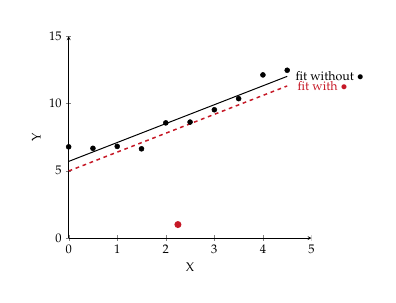
\begin{tikzpicture}[scale=0.45]
% For the regression graph below
\pgfmathsetseed{1146} % set the random seed
\pgfplotstableset{ % Define the equations for x and y
	create on use/x/.style={create col/expr={\pgfplotstablerow/2}},
	create on use/y/.style={create col/expr={1.3*\thisrow{x} + 5.5 + 1.5*rand}}
}
% create a new table with 10 rows and columns x and y:
\pgfplotstablenew[columns={x,y}]{10}\loadedtable
\begin{axis}[
xlabel=X, % label x axis
ylabel=Y, % label y axis
axis lines=left, %set the position of the axes
xmin=0, xmax=5, % set the min and max values of the x-axis
ymin=0, ymax=15, % set the min and max values of the y-axis
clip=false
]

%\pgfplotstablesave{\loadedtable}{../Tables/Tab09.dat}

\addplot [only marks] table {\loadedtable};
\addplot [no markers, thick, title] table [y={create col/linear regression={y=y}}] {\loadedtable} node[xshift=1.2cm] {fit without $\bullet$};
\node [circle, fill=title, color=title, inner sep=-2pt] (A) at (225,10) {};
\draw[very thick, dashed, color=title] (0, 49.80074)--(450,113.05366) node[xshift=1cm] {fit with $\bullet$};
\end{axis}
\end{tikzpicture}
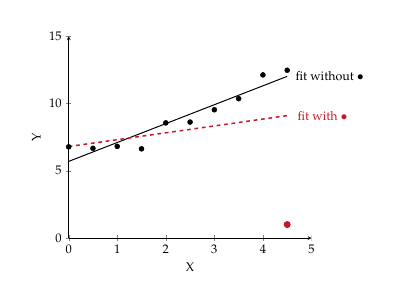
\begin{tikzpicture}[scale=0.45]
% For the regression graph below
\pgfmathsetseed{1146} % set the random seed
\pgfplotstableset{ % Define the equations for x and y
	create on use/x/.style={create col/expr={\pgfplotstablerow/2}},
	create on use/y/.style={create col/expr={1.3*\thisrow{x} + 5.5 + 1.5*rand}}
}
% create a new table with 10 rows and columns x and y:
\pgfplotstablenew[columns={x,y}]{10}\loadedtable
\begin{axis}[
xlabel=X, % label x axis
ylabel=Y, % label y axis
axis lines=left, %set the position of the axes
xmin=0, xmax=5, % set the min and max values of the x-axis
ymin=0, ymax=15, % set the min and max values of the y-axis
clip=false
]

\addplot [only marks] table {\loadedtable};
\addplot [no markers, thick, title] table [y={create col/linear regression={y=y}}] {\loadedtable} node[xshift=1.2cm] {fit without $\bullet$};
\node [circle, fill=title, color=title, inner sep=-2pt] (A) at (450,10) {};
\draw[very thick, dashed, color=title] (0, 68,857)--(450,91,90272) node[xshift=1cm] {fit with $\bullet$};
\end{axis}
\end{tikzpicture}
\centering
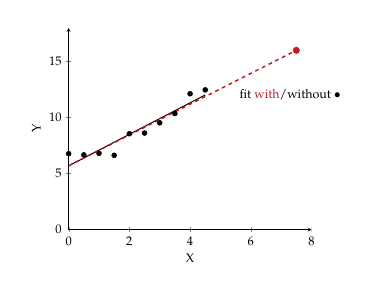
\begin{tikzpicture}[scale=0.45]
% For the regression graph below
\pgfmathsetseed{1146} % set the random seed
\pgfplotstableset{ % Define the equations for x and y
	create on use/x/.style={create col/expr={\pgfplotstablerow/2}},
	create on use/y/.style={create col/expr={1.3*\thisrow{x} + 5.5 + 1.5*rand}}
}
% create a new table with 10 rows and columns x and y:
\pgfplotstablenew[columns={x,y}]{10}\loadedtable
\begin{axis}[
xlabel=X, % label x axis
ylabel=Y, % label y axis
axis lines=left, %set the position of the axes
xmin=0, xmax=8, % set the min and max values of the x-axis
ymin=0, ymax=18, % set the min and max values of the y-axis
clip=false
]

\addplot [only marks] table {\loadedtable};
\addplot [no markers, thick, title] table [y={create col/linear regression={y=y}}] {\loadedtable} node[xshift=2.4cm] {fit \textcolor{title}{with}/without $\bullet$};
\node [circle, fill=title, color=title, inner sep=-2pt] (A) at (750,160) {};
\draw[very thick, dashed, color=title] (0, 57,40234)--(750,160,97071);
\end{axis}
\end{tikzpicture}
\caption{\footnotesize{\textbf{Left panel}: Outlier, but with low leverage. \textbf{Center panel}: Outlier, with high leverage. \textbf{Right panel}: High leverage, but not an outlier.}}
\end{figure}

\end{frame}




\begin{frame}{Influence on coefficients}

  \begin{equation}
Influence = Leverage \times Discrepancy
  \end{equation}

  The case in the second panel has high influence (on the regression slope).\bigskip

  The case in the third panel is nevertheless problematic.

  \begin{equation}
    V(b) = \frac{\sigma_\epsilon^2}{\sum_{i=1}^n(x_i - \bar{x})^2}
  \end{equation}

  The sampling variance is ``artificially'' reduced in such cases.

\end{frame}





\section{Additional assumptions}

\begin{frame}
\begin{center}
    \Huge Additional assumptions
\end{center}
\end{frame}


\begin{frame}{Other assumptions}
Encountered frequently \cite{berry1993}, but without a clear solution:

\begin{itemize}
\item some depend on the researcher's background knowledge, and not on a statistical fix, e.g. measurement error;
\item for others the solutions are not straightforward, and sometimes depend on learning more advanced procedures, e.g. collinearity.
\end{itemize}

\end{frame}


\subsection{No specification error}

\begin{frame}{No specification error}
The assumption requires that the estimated model is \textit{complete}: excludes variables that ought not to be there, and includes all variables that ought to be there.\bigskip

Theory provides a list of variables.\bigskip

Take an example. Although the full model is:

\begin{equation}
Y = a + b_{11}X_1 + b_{12}X_2 + \epsilon_1
\end{equation}

we can only test:

\begin{equation}
Y = a + b_{21}X_1 + \epsilon_2
\end{equation}

\end{frame}



\begin{frame}{Effects of mis-specification}
Further assume that $X_1$ and $X_2$ are weakly correlated.\bigskip

\begin{itemize}
\item $X_2$ excluded from the model
\item $X_2$ is correlated with $X_1$
\item $X_2$ has a partial effect on $Y$
\end{itemize}

The effect of $X_2$ is now part of $X_1$ $\Rightarrow$ $b_{21} \neq b_{11}$.

\end{frame}



\begin{frame}{Diagnosis}
There is a test: Ramsey's RESET (Regression Equation Specification Error Test).\bigskip

This is limited, as it only refers to functional specification, and tests for any omitted non-linear predictors.\bigskip

Ultimately, it's down to knowing the theory and having the right data available.

\end{frame}



\subsection{No measurement error}

\begin{frame}{No measurement error (in the predictors)}
Measurement error in the outcome can be accommodated in OLS.\bigskip

$e_i$ have a non-normal distribution, but $a$ and $b$s are still BLUE (\textit{Best Linear Unbiased Estimators}).\bigskip

BLUE requires only the assumption of linearity, homoskedasticity, and error independence.\bigskip

Measurement in the predictors, though, impacts the estimates.

\end{frame}


\begin{frame}{No measurement error (in the predictors)}
Measurement error in the predictors tends to bias coefficients downward (they are smaller than they should be).\bigskip

Ultimately, probably all indicators have some measurement error to them.\bigskip

Two aspects are important:

\begin{itemize}
\item the size of the error;
\item whether it's random or systematic.
\end{itemize}

\end{frame}



\begin{frame}{No measurement error (in the predictors)}
Random error $\Rightarrow$ $a$ and $b$s are unbiased, but SEs are larger, and $R^2$ is lower \cite[p.~51]{berry1993}.\bigskip

Systematic error $\Rightarrow$ even the $a$ and $b$s are biased.\bigskip

No magic bullet: put a lot of time in concept operationalization.\bigskip

\end{frame}





\subsection{No autocorrelation}

\begin{frame}{No autocorrelation}
Particularly salient in time-series analysis.\bigskip

$e_t$ tends to correlate with $e_{t+1}$ because some phenomena exhibit slow change and multi-year trends (e.g. unemployment, GDP/capita).\bigskip

A test is available: the Durbin-Watson test.\bigskip

\begin{equation}
  D = \frac{\sum_{t=2}^n(\epsilon_t - \epsilon_{t-1})^2}{\sum_{t=1}^n\epsilon_t^2}
\end{equation}
\end{frame}


\begin{frame}{No autocorrelation}

For a large $n$, $D \approx 2(1-\rho)$, where $\rho$ is the correlation coefficient between $\epsilon_t$ and $\epsilon_{t+1}$.\bigskip

A $D \approx 2$ suggests that $\rho \approx 0$, which is ideal.\bigskip

The limits of $D$ are 0, when $\rho=1$, and 4, when $\rho=-1$.

\end{frame}



\subsection{No (perfect) collinearity}

\begin{frame}{No (perfect) collinearity}

The formula for sampling variance of a particular predictor, $X_j$, in multiple regression had the VIF:

\begin{equation}
VIF = \frac{1}{1 - R_j^2}
\end{equation}

$R_j^2$ is the model fit from a regression of $X_j$ on all the other predictors in the model.\bigskip

The higher the correlation between $X_j$ and another predictor, the higher the $R_j^2$ $\Rightarrow$ high VIF $\Rightarrow$ high sampling variance.

Large SEs means that there isn't enough (independent) information to properly estimate $b$.
\end{frame}


\begin{frame}{Solutions: high collinearity}

Yet again, no magic bullet:

\begin{itemize}
\item create an index, if it's theoretically plausible;
\item drop a variable from the model, and risk mis-specification error;
\item collect more data, to estimate $b$ with more precision;
\item ridge regression: accept a bit of bias in your coefficients, for a larger gain in efficiency.
\end{itemize}

\end{frame}



% FRAME
\begin{frame}
\begin{center}
    \Huge Thank \textcolor{title}{you} for the kind attention!
\end{center}
\end{frame}

% REFERENCES %

\begin{frame}[allowframebreaks]{References}
\bibliographystyle{apacite}
\bibliography{../Bibliography}
\end{frame}

\end{document}
